\documentclass{scrartcl}
\usepackage{german}
\usepackage[T1]{fontenc}
\usepackage[utf8]{inputenc}
\usepackage[german]{babel}

% zusätzliche mathematische Symbole, AMS=American Mathematical Society
\usepackage{amssymb}

% fürs Einbinden von Graphiken
\usepackage{graphicx}

% für Namen etc. in Kopf- oder Fußzeile
\usepackage{fancyhdr}

% erlaubt benutzerdefinierte Kopfzeilen
\pagestyle{fancy}

% Definition der Kopfzeile
\lhead{
	\begin{tabular}{ll}
		Fisnik Zeqiri & 4306430 \\
		Felix  Karg   & 4342014
	\end{tabular}
}
\chead{}
\rhead{\today{}}
\lfoot{}
\cfoot{Seite \thepage}
\rfoot{}

\begin{document}
	\section*{Lösungen zum Übungsblatt Nr. 2}

	\subsection*{Aufgabe 1}

		\begin{table}[h]

			\begin{tabular}{c|c|c}
				PC & ReTI & Kommentar \\
				\hline
				0 & LoadI 1 &  \\
        1 & Store 0 & Zellen 0 und 1 werden auf 1 gesetzt \\
				2 & Store 1 &  (Ersten beiden Fibonacci-Zahlen) \\ \hline
				3 & Jump LE 12 & prüfen ob \(n\le0\) ist (außer beim ersten Durchgang,\\&& da ist ACC=1 statt $n$) \\ \hline
				4 & Load 0 &  \\
        5 & Add 1 & S(0) wird um den wert von S(1) erhöht \\
				6 & Store 2 & und in S(2) gespeichert \\ \hline
        7 & Load 1 & S(1) überschreibt S(0). \\
				8 & Store 0 & \\% Zelle 0 wurde im vorherigen schritt auf Zelle 2 gespeichert \\ \hline
        9 & Load 2 & S(2) überschreibt S(1) \\
				10 & Store 1 &  \\ \hline
				11 & Load 30 &  \\
        12 & SubI 1 & von S(30) ($n$) wird 1 abgezogen \\
				13 & Store 30 &  \\ \hline
				14 & Jump -11 & zu Zeile 3, Bedingungslos \\ \hline
				15 & Load 0 &  Die Aktuelle Fibonacci-Zahl wird geladen \\
				16 & Store 33 & und in Zelle 33 gespeichert \\
			\end{tabular}
		\end{table}

Der Aktuelle wert der $n$-ten Fibonacci-Zahl ist in S(0). S(30) ist der aktuelle wert von $n$.
Er wird vor der Schleife immer um 1 Subtrahiert,
bis er die Bedingung für die schleife nicht mehr erfüllt ($\le0$).
In den letzten beiden Schritten wird der wert von S(0) in S(33) (ergebnis) gespeichert.


	\subsection*{Aufgabe 2}
	\begin{itemize}
		\item[a)] Häufigkeitsverteilung:
		 \begin{table}[h]
			\begin{tabular}{c|c|c|c|c|c|c|c|c|c|c|c}

				I & T & F & U & N & R & K & M & A & E & O & S \\ \hline
				4 & 4 & 2 & 2 & 2 & 2 & 1 & 1 & 1 & 1 & 1 & 1 \\
			\end{tabular}
		\end{table}

	 	\newpage
	 	\item[b)] Huffman-Code\\ 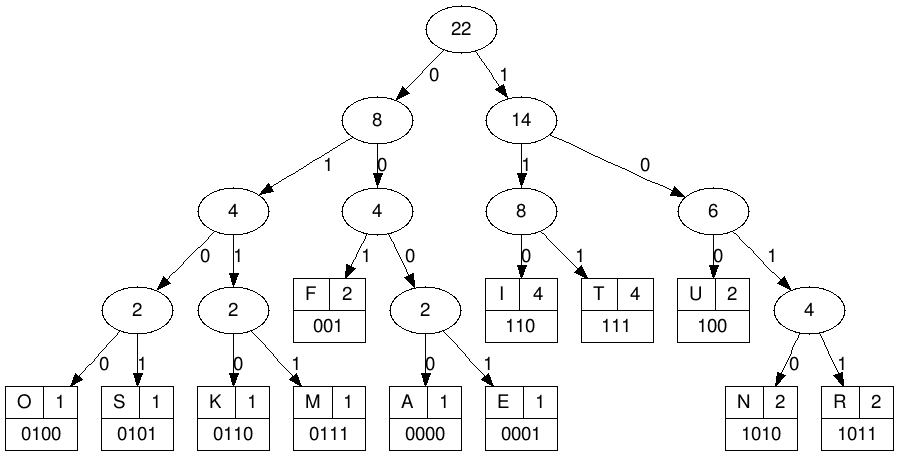
\includegraphics[width=13cm]{tree.png}

	 	\item[c)] Kodierter Text \\
	 	110 1010 0101 111 110 111 100 111 001 100 0001 1011 110 1010 001 0100 1011 0111 0000 111 110 0101 \\
    (Stream: 1101010010111111011110011100110000011011110101000101001011011100001111100101) \\
	 	\item[d)] Unterschiedliche Kodierung\\
	 	Eine unterschiedliche Kodierung muss nicht zwangsläufig heißen, dass jemand einen Fehler gemacht hat.
    Es gibt mehrere Buchstaben mit derselben Häufigkeit, die man auch unterschiedlich miteinander verknüpfen kann.
    Es spielt keine Rolle welche gleichhäufigen Buchstaben man miteinander verknüpft.
	\end{itemize}

	\subsection*{Aufgabe 3}
	Z.z: S(2) = x*y \\
	IA: F(x,0) = x*0 = 0 \\
  Erst wird $0$ in S(2) geschrieben, dann wird von $y$ $1$ abgezogen und geprüft ob $y < 0$ ist.
  Da dies der Fall ist, ist das Programm zu Ende, und Richtig da das Ergebnis
  $x * 0 = 0$ in S(2) ist.  \\
	IV: F(x,y) = $x * y$ \\
	IS: F(x,y+1) = $x * (y + 1)$ \\
	Das Ergebnis wird auf $0$ gesetzt und von y wird 1 abgezogen.
  Da y nicht < 0 ist, wird das Ergebnis geladen, $1 * x$ addiert und gespeichert.\\
	Da im folgenden nur noch $x * y$ (IV) zum Ergebnis ($1 * x$) addiert wird, ist das
  Endergebnis also $x * y + x = x * (y + 1)$. \hfill $\Box$

\newpage
	\subsection*{Aufgabe 4}
      Sei ein Element entweder ein Buchstabe $a_n$ des Alphabets oder ein Binärer Baum mit
      der Summe der Wsk seiner Elemente als Wsk. \\
  \begin{itemize}
    \item[a)] Da es mindestens 3 Elemente gibt, Element $a_i$ allein bereits $> 50\%$ Wsk
      (=Wahrscheinlichkeit(/en)) hat, und immer Zwei Elemente mit den niedrigsten Wsk verbunden werden,
      Wird das Element $a_i$ zwingend als letztes mit dem Rest-Baum der alle anderen Beinhaltet verbunden,
      da es erst dann 'eines der kleinsten' ist, dadurch bekommt es je nach Reihnfolge entweder die
      $1$ oder die $0$, und alle anderen ein präfix mit dem Inversen davon.
      \hfill $\Box$ \\ \\


    \item[b)]
      Angenommen es gibt ein $a_i$ mit $|c(a_i)| = 1$ hat $p(a_i) < 1/3$. \\
      Beim Aufbauen des Huffman-Codes Werden bekanntermaßen immer die Kleinsten Zwei Elemente
      verknüpft, und angenommen unser $a_i$ schafft es bei den Letzten drei Elementen noch nicht
      verknüpft zu sein. Dann gibt es Folgende möglichkeiten:
      \begin{itemize}
        \item[1)] $p(a_i)$ ist kleiner als die Wsk der beiden anderen Elemente,
          wodurch es ausgewählt wird und im vorletzten schritt schon länge 1 hat, wodurch
          es insgesamt in Schritt 2 länge 2 bekommt. Da $|c(a_i)| = 1$ ist ist dies offensichtlich Falsch.
        \item[2)] $p(a_i)$ ist die zweitkleinste Wsk, auch jetzt wird es ausgewählt und bekommt
          eine länge von 2. Da $|c(a_i)| = 1$ ist ist dies offensichtlich Falsch.
        \item[3)] $p(a_i)$ hat mit $< 1/3$ die größte Wsk der verbleibenden drei Elemente. Das kann nicht sein,
          da die Summe der Wsk 1 ergeben muss, und \(\forall_{b < 1/3} 3 * b < 1\) gilt.
        \item[4)] Alle Drei verbleibenden Elemente haben die gleiche Wsk. Analog vorhergehende Begründung.

        \item[5)] $p(a_i)$ ist gleich groß wie die Wsk eines anderen Elements. Da Bereits zwei Elemente
          die Wsk $< 1/3$ haben, muss zwingend das letzte Größer sein, in diesem Fall siehe
          Begründung 1 oder 2.
      \end{itemize}
      Da alle möglichkeiten eines Buchstabens mit $p(a_i) < 1/3$ eine Länge von $|c(a_i)| = 1$ zu haben
      anscheinend nicht möglich sind, ist der zwingend Folgende schluss dass unsere Annahme nicht gelten kann
      und damit die Negation unserer Annahme gilt,
      also dass \(\forall_{a_i \in A}: p(a_i) \geq 1/3\) gelten muss, wenn $|c(a_i)| = 1$. \hfill $\Box$


  \end{itemize}







\end{document}
